%========================================================================
% Modelo para elaboracao de textos academicos: TCC, dissertacoes e teses
% Elaborado pelo GISIS - Grupo de Imageamento Sismico e Inversao Sismica.
%========================================================================
\chapter{Discussões}
\label{ch:discussoes}

% Focar nos impactos da imprecisão no cálculo dos tempos na inversão
% Analisar as diferenças e ruídos de inversão para cada método
% Analisar performance em relação aos resultados
 
Neste capítulo, os comentários acerca dos resultados são desenvolvidos em duas etapas. Primeiro, uma análise dos métodos de modelagem em relação a performance e precisão é realizada e segundo, os resultados da tomografia são discutidos.   
 
\section{Análise da precisão e performance} 

No teste do modelo homogêneo (Tabela \ref{table_homog}) nota-se a superioridade em performance do método de \citeonline{jeong2008fast}, porém os erros registrados são os mais altos em relação aos outros métodos testados. O método de \citeonline{cai2023improved} consegue reduzir o erro do \textit{Fast Iterative Method}, contudo, além de não ser o mais preciso entre os métodos analisados, a nova formulação se mostrou performaticamente inferior em relação às demais estudadas. O método que demonstrou mais precisão foi a nova implementação do \textit{Fast Sweeping Method} utilizando a estratégia de paralelização de \citeonline{detrixhe2013parallel} e os operadores desenvolvidos no trabalho de \citeonline{noble2014accurate}. A eficiência computacional do \textit{Fast Sweeping Method} não se destacou como a mais performática, porém se demonstra promissora ao considerar o conjunto entre precisão e performance.  

A solução clássica demonstrou desempenho computacional razoável para problemas pequenos, porém quando a dimensão do problema aumenta os tempos de execução não se adequam aos demais métodos, embora tenha boa precisão. O exemplo utilizando o modelo de duas camadas mostra que a performance da formulação de \citeonline{podvin1991finite} diminui consideravelmente, no modelo com 25 m de discretização, enquanto as demais mantêm seus patamares abaixo de um segundo de tempo de execução. Em relação à precisão, novamente a metodologia de \citeonline{noble2014accurate} demonstra superioridade sendo que o máximo erro absoluto registrado não passou de 5 ms, enquanto os erros máximos absolutos de 120 e 350 ms foram registrados para os métodos de \citeonline{podvin1991finite} e \citeonline{jeong2008fast}, respectivamente. O dado de reciprocidade gerado com o modelo de 25 m foi respeitado em todos os métodos testados. Embora inicialmente o \textit{Fast Sweeping Method} tenha atribuído erros aos tempos recíprocos, o problema de inicialização foi resolvido e a precisão foi mantida. As máximas diferenças em relação à equação analítica registradas para o modelo de duas camadas (Figura \ref{fig:precision_refraction_study}) foram de -40, -100 e -2 ms para as formulações clássica, \textit{Fast Iterative Method} e \textit{Fast Sweeping Method}, respectivamente.         

A aplicação dos métodos no modelo complexo foi realizada com sucesso, então, os tempos de trânsito (Figuras \ref{fig:overthrust_inner_circle}, \ref{fig:overthrust_mid_circle} e \ref{fig:overthrust_outer_circle}) e de execução (Tabela \ref{table_overthrust}) foram registrados. Novamente, o método clássico demonstrou tempo de execução acima dos demais para problemas grandes. O método de \citeonline{jeong2008fast} demonstra eficiência computacional e o \textit{Fast Sweeping Method} performa 26$\%$ abaixo do método mais performático. Considerando o ganho de precisão, a diferença de performance pode ser desconsiderada pois \citeonline{cai2023improved} mostram a utilização do método original de \citeonline{jeong2008fast} na migração Kirchhoff em profundidade, onde os erros de posicionamento dos refletores são amplamente perceptíveis. Os tempos de trânsito ilustrados nas Figuras \ref{fig:overthrust_inner_circle}, \ref{fig:overthrust_mid_circle} e \ref{fig:overthrust_outer_circle} mostram as discrepâncias entre os métodos aplicados ao modelo SEG/EAGE \textit{Overthrust}, sendo que os atrasos percebidos na Figura \ref{fig:precision_refraction_study} se repetem, porém no modelo complexo. Se mostra visível nas Figuras \ref{fig:overthrust_inner_circle}, \ref{fig:overthrust_mid_circle} e \ref{fig:overthrust_outer_circle} os detalhes que o modelo impõe aos tempos de trânsito, nas formulações de \citeonline{podvin1991finite} e \citeonline{noble2014accurate}, e a falta de definição para a formulação menos precisa de \citeonline{jeong2008fast}.  
 
\section{Análise dos resultados da tomografia} 
 
Os artifícios da análise dos resultados foram organizados esquematicamente baseados na Figura \ref{fig:discuss_geometry}. Como os dados estão ordenados no domínio do receptor, linhas de tiros foram registradas utilizando tanto os modelos recuperados por malha esparsa quanto por malha refinada. Após a recuperação dos modelos, a modelagem serviu de ferramenta para gerar os dados para cada formulação que resolve a equação eikonal. O receptor em questão para as análises está destacado em vermelho e as linhas em azul na Figura \ref{fig:discuss_geometry}. O domínio do modelo também foi explorado com cinco perfis de velocidade nas posições em lilás na Figura \ref{fig:discuss_geometry}, esses pontos são os mesmos que geraram a superfície alvo (Tabela \ref{target_gaussian_coefs}). As análises no domínio do tempo estão ilustradas nas Figuras \ref{fig:zoom_out} e \ref{fig:zoom_in}, e no domínio do modelo são mostradas na Figura \ref{fig:model_profile}. 
 
\begin{figure}[H]
	\centering
	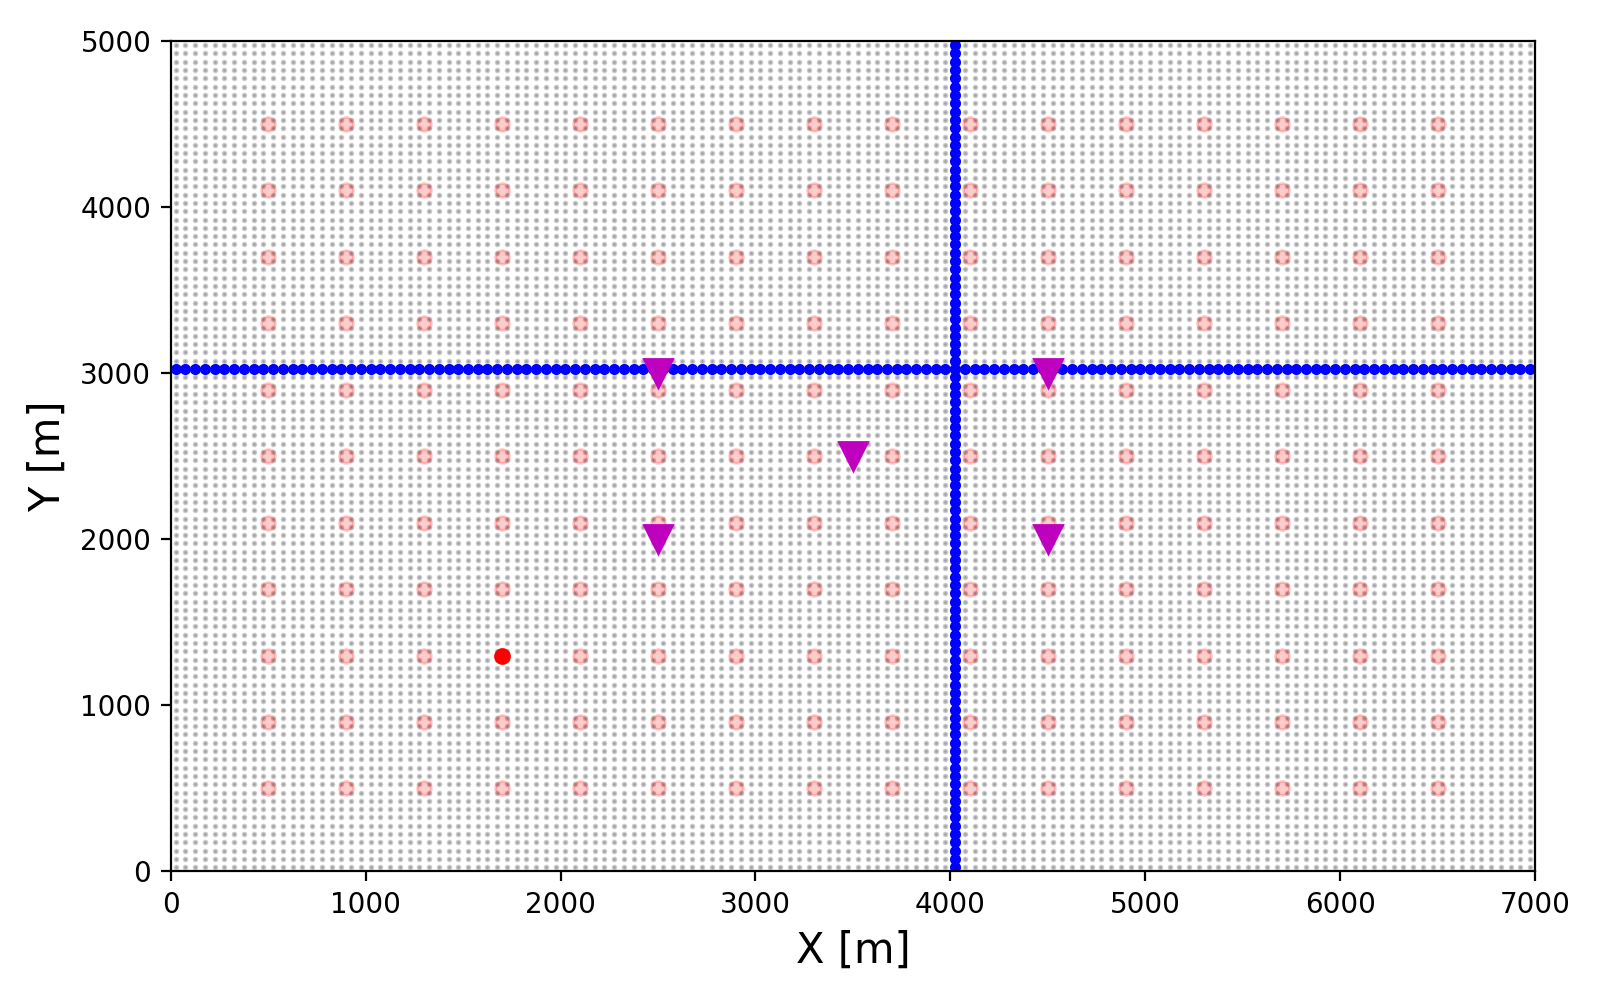
\includegraphics[width=12cm,height=7cm]{Imgs/Discussoes/discuss_geometry.png}
	\caption{Panorama de discussão envolvendo o dado e os modelos. Em relação aos dados, que estão ordenados no domínio do receptor, o ponto vermelho de tonalidade marcante será o receptor de referência. Os pontos azuis em destaque são as linhas de tiros utilizadas apara a análise. Em relação ao modelo, cinco pontos (triângulo invertido de cor lilás) foram destacados nas mesmas posições das gaussianas utilizadas para gerar o modelo de referência.}
	\label{fig:discuss_geometry}	
\end{figure}

\begin{figure}[H]
	\centering
	\subfloat[]{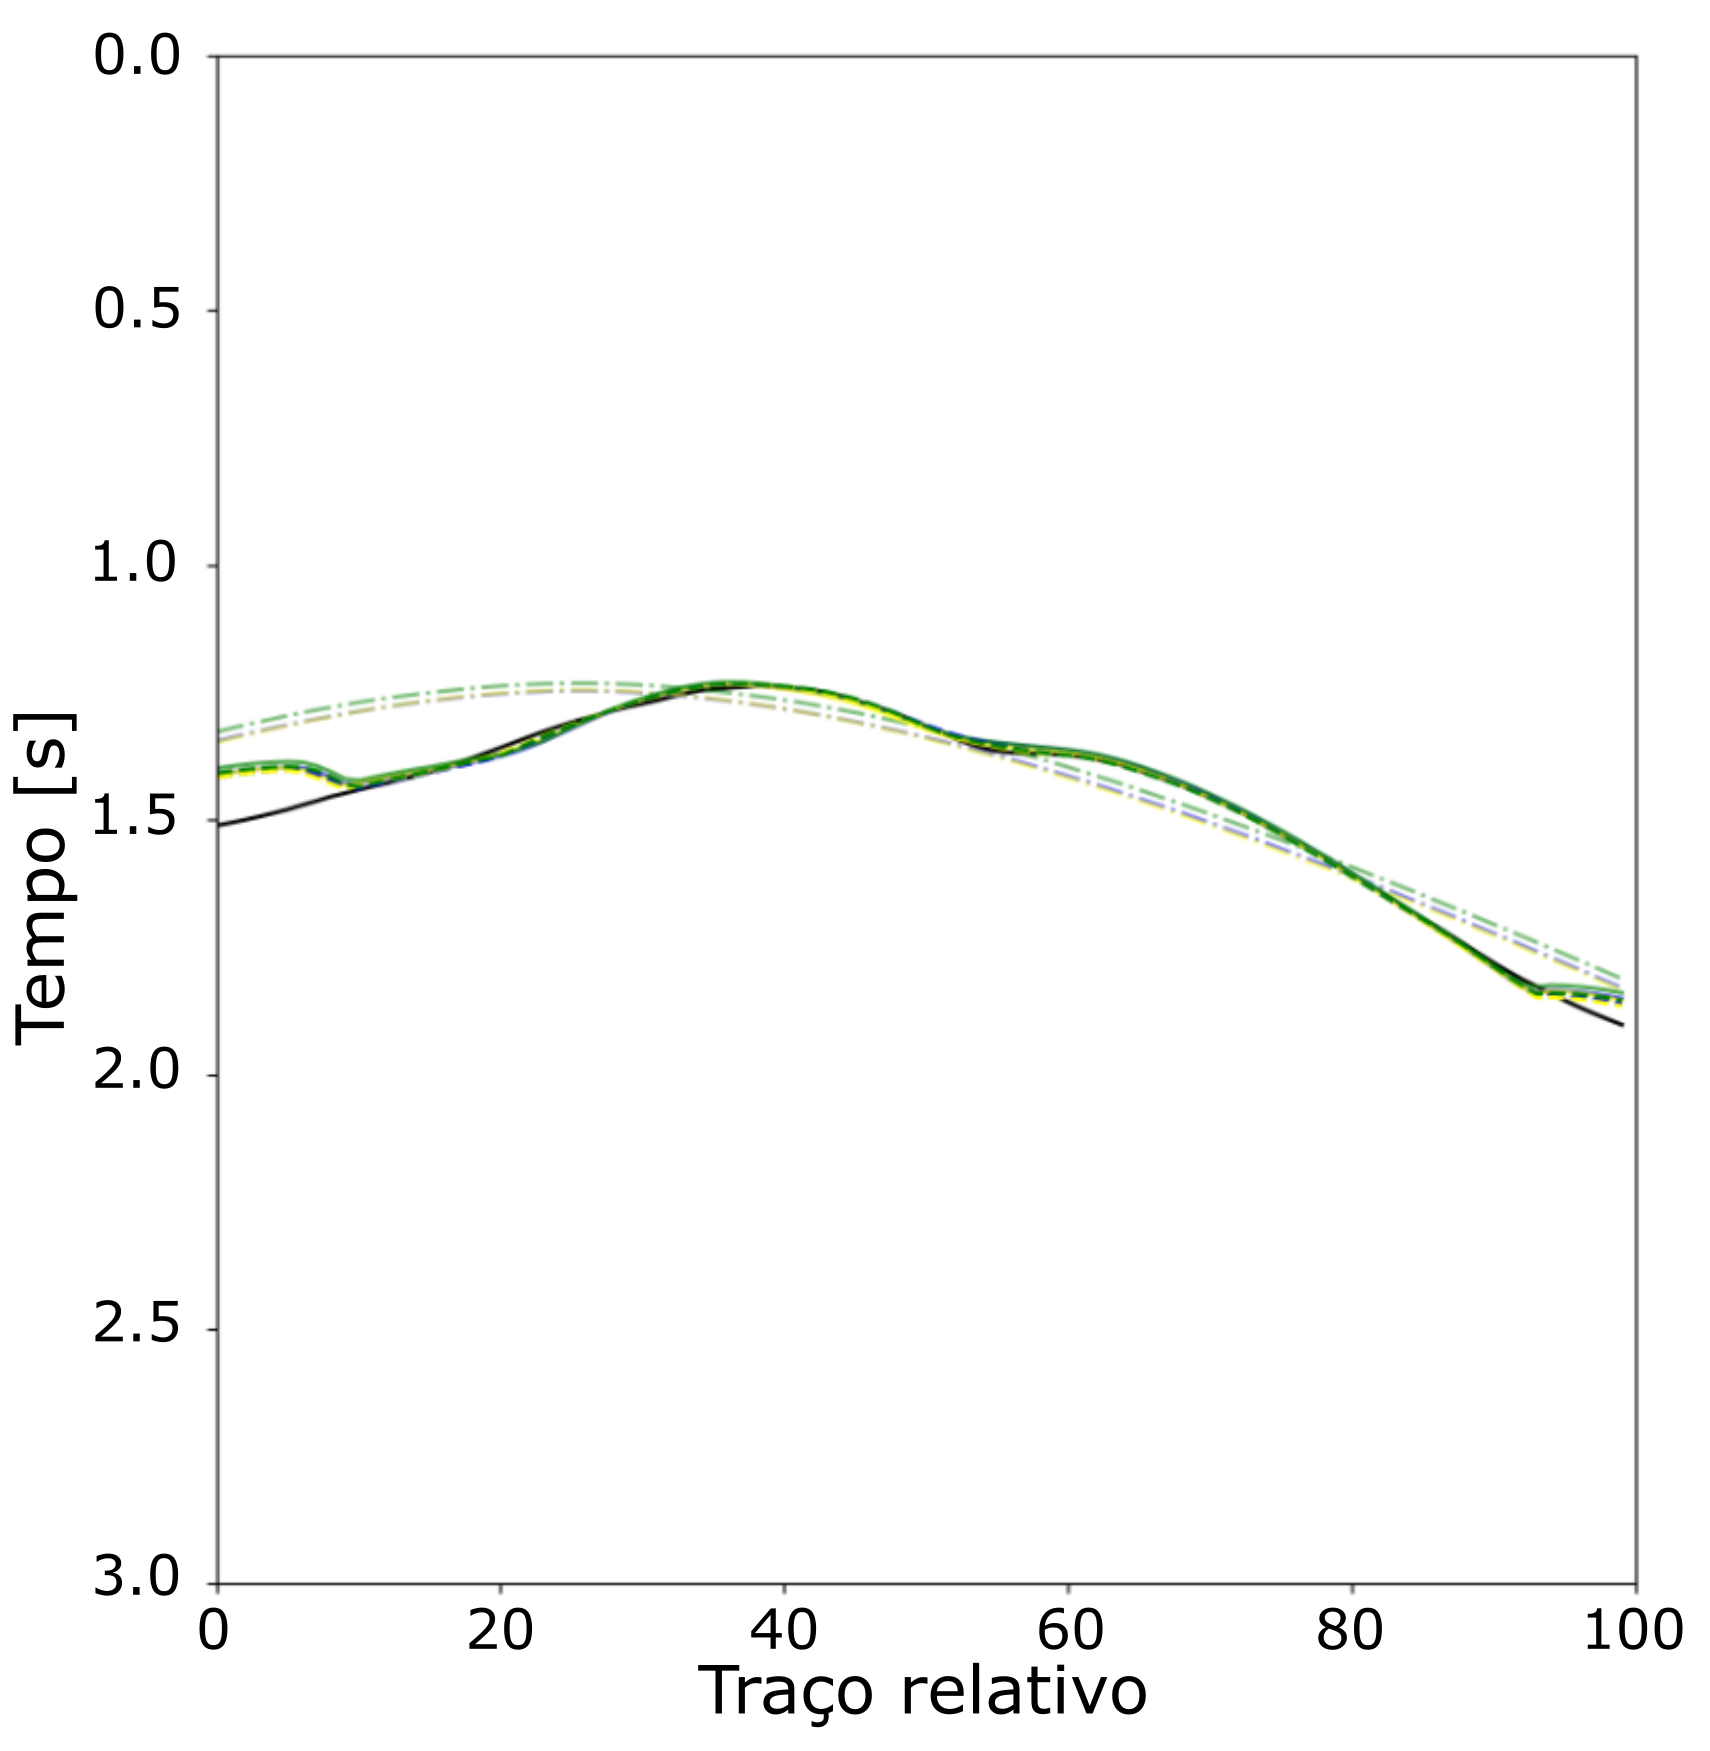
\includegraphics[width=8cm,height=9cm]{Imgs/Discussoes/xz_zoom_out.png}}
	\subfloat[]{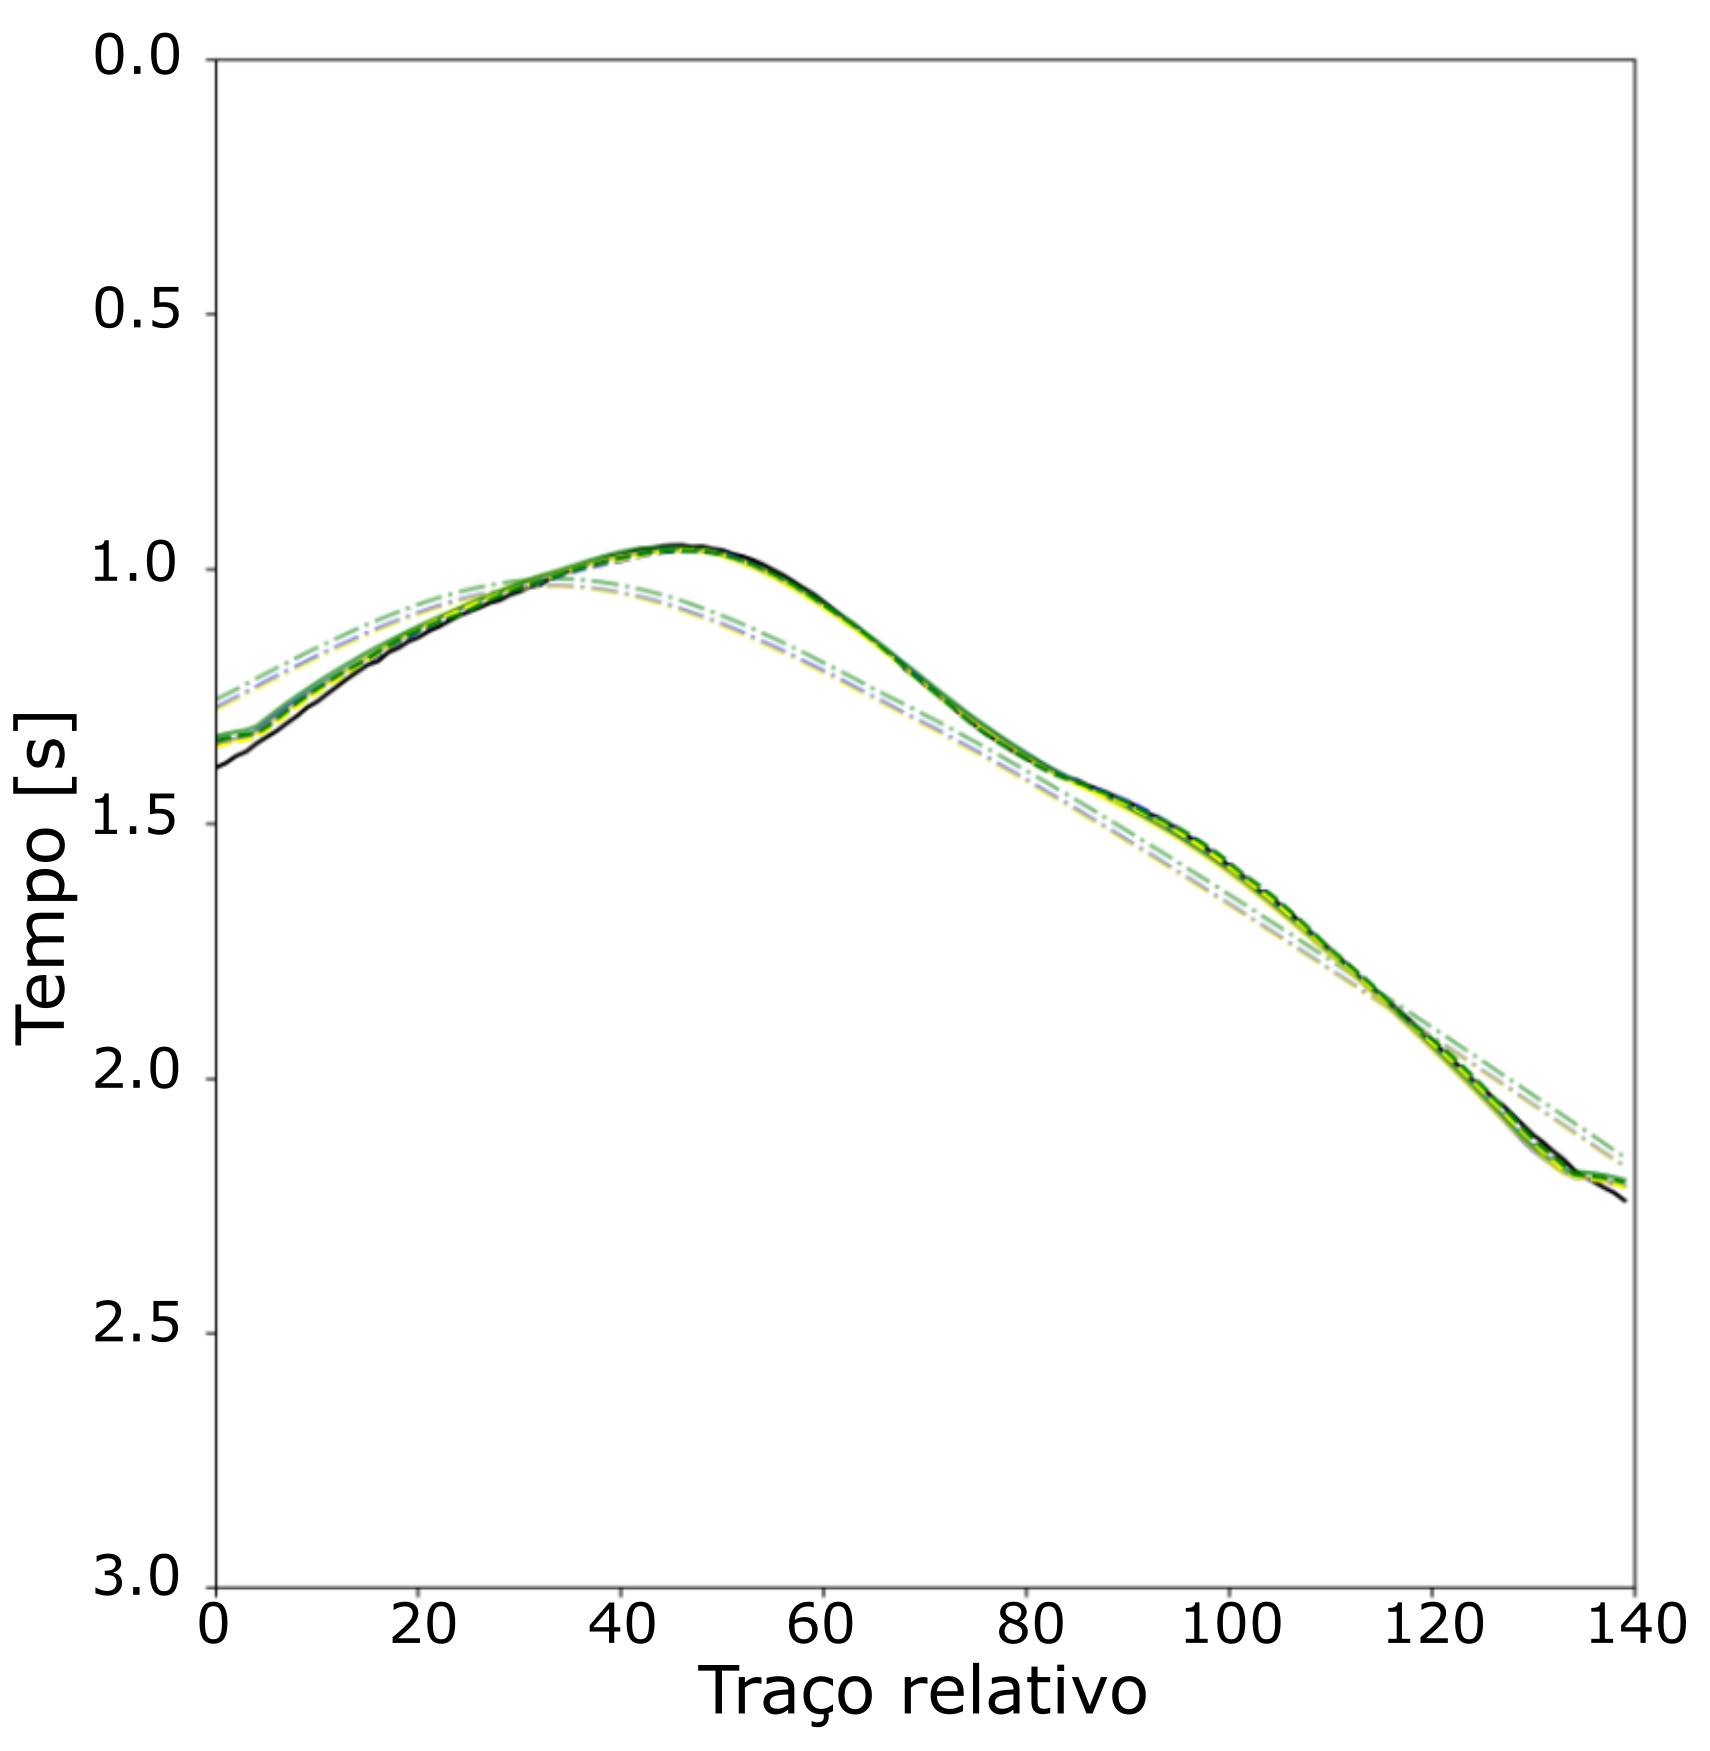
\includegraphics[width=8cm,height=9cm]{Imgs/Discussoes/yz_zoom_out.png}}
	
	\caption{Comparação de dados incluindo o dado observado (linha preta sólida), dado inicial (linhas coloridas opacas com traço e ponto), dado gerado a partir do primeiro processo de inversão (linhas coloridas sólidas) e o dado gerado a partir do segundo processo de inversão (linhas coloridas tracejadas). Em relação aos métodos estudados, a cor azul se refere à formulação de \citeonline{podvin1991finite}, a cor amarela \citeonline{jeong2008fast} e a cor verde \citeonline{jeong2008fast}.}
	\label{fig:zoom_out}
\end{figure}

De maneira geral, em relação ao ajuste dos dados, a Figura \ref{fig:zoom_out} mostra que a partir de um dado completamente deformado (linhas tracejadas opacas) a tomografia consegue diminuir a diferença entre dado calculado e observado (linha preta). Algumas regiões não foram bem ajustadas por consequência da limitação do modelo de velocidade no momento da atualização, negligenciando 200 m nas extremidades das direções $x$ e $y$. Esse detalhe é bem representado na Figura \ref{fig:zoom_out}a, na parte esquerda do dado.  

Observando o detalhe, a Figura \ref{fig:zoom_in}a ilustra as diferenças do ajuste dos dados utilizando a malha esparsa (linhas sólidas) e a malha refinada (linhas tracejadas). Realmente, a inversão de malha refinada consegue ajustar os dados ao ponto de atingir melhor definição que a inversão de malha esparsa, contudo grandes diferenças ainda podem ser observadas principalmente na parte central da Figura \ref{fig:zoom_in}a. Embora grandes diferenças no ajuste do dado observado e calculado após os processos de inversão sejam menos impactantes, a Figura \ref{fig:zoom_in}b ainda mostra os detalhes aprimorados do dado calculado diante da redução da malha na inversão.

\begin{figure}[H]
	\centering
	\subfloat[]{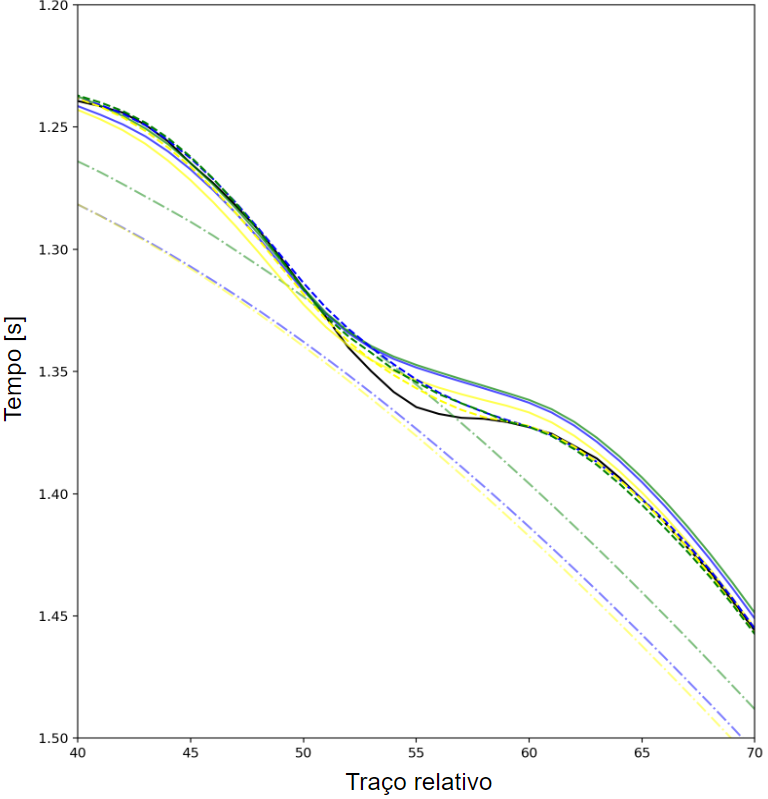
\includegraphics[width=8cm,height=9cm]{Imgs/Discussoes/xz_zoom_in.png}}
	\subfloat[]{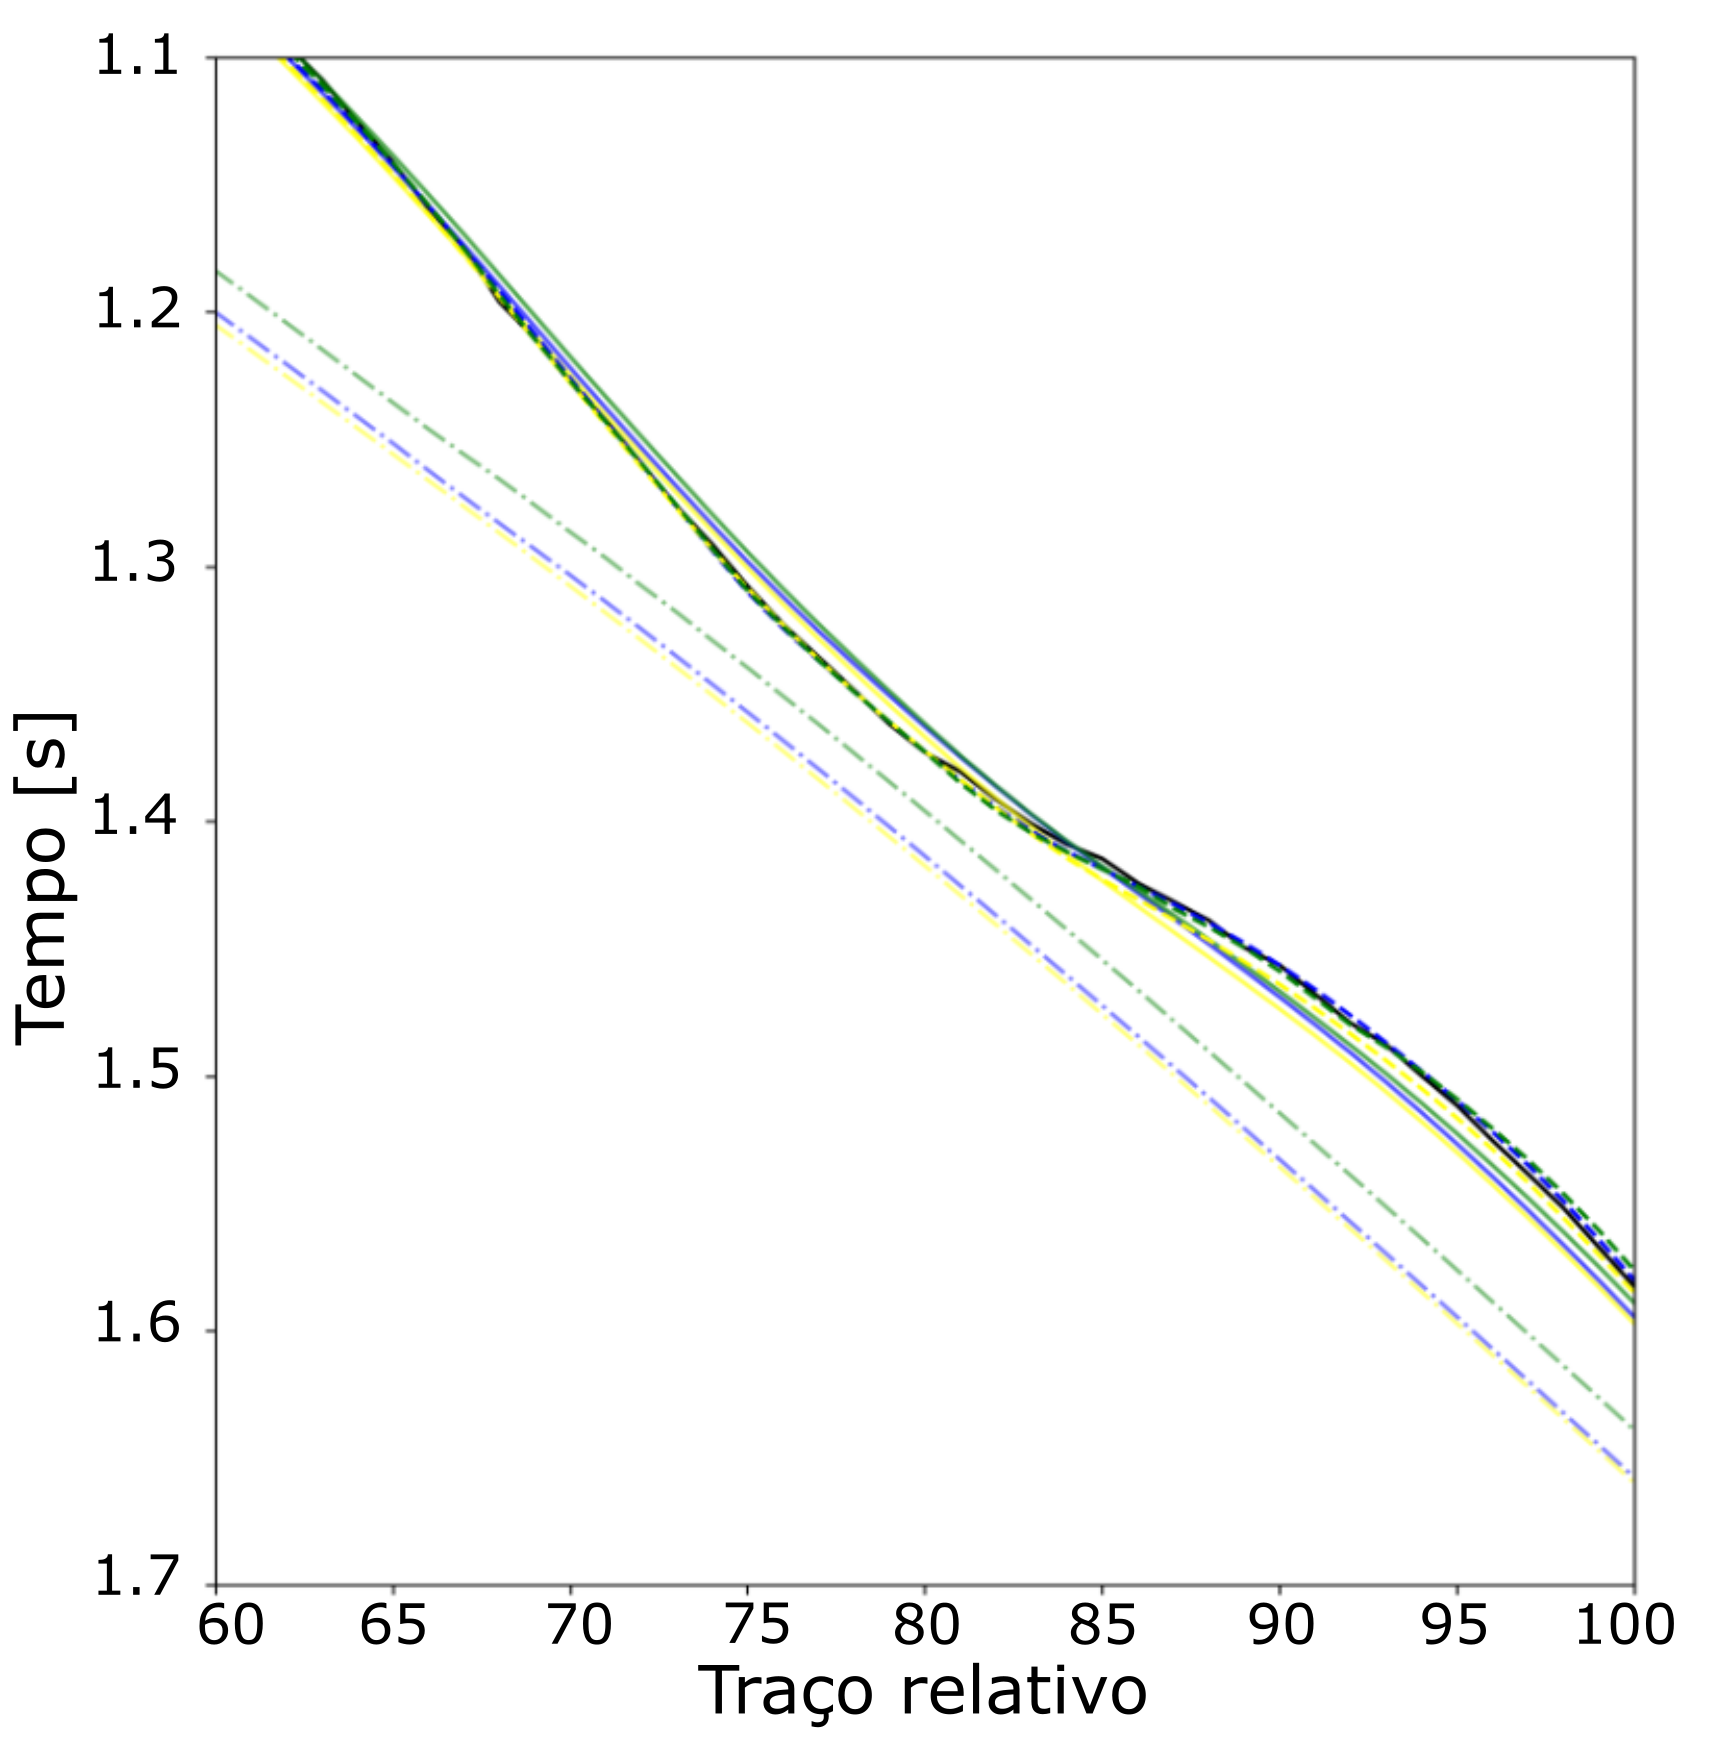
\includegraphics[width=8cm,height=9cm]{Imgs/Discussoes/yz_zoom_in.png}}
	
	\caption{Aproximação para melhor análise dos dados. Dado observado se apresenta como a linha preta sólida, o dado inicial, linhas coloridas com traço e ponto, dado gerado com modelo da inversão esparsa, linhas coloridas sólidas, e o dado gerado com modelo da inversão refinada, linhas coloridas tracejadas. Em relação aos métodos estudados, a cor azul se refere à formulação de \citeonline{podvin1991finite}, a cor amarela \citeonline{jeong2008fast} e a cor verde \citeonline{jeong2008fast}.}
	\label{fig:zoom_in}
\end{figure}

As atualizações do modelo de velocidade projetadas em perfis são ilustradas na Figura \ref{fig:model_profile}, sendo as linhas pretas e vermelhas referentes aos modelos de referência e inicial, respectivamente. De maneira geral as linhas que representam os modelos recuperados utilizando os diferentes algoritmos de modelagem não apresentaram variações marcantes para cada método de resolução eikonal. Ilustrado na Figura \ref{fig:model_profile}, as linhas sólidas opacas representam a projeção em perfil dos modelos recuperados utilizando malha esparsa e as linhas tracejadas são os resultados finais dos modelos recuperados com malha refinada. Pode-se observar, na Figura \ref{fig:model_profile}a e \ref{fig:model_profile}e, o aumento da definição do modelo após o refinamento da malha de inversão, nas profundidades entre 700 e 900 metros. A suavidade é notada em todas as regiões selecionadas e a tomografia não conseguiu recuperar os altos contrastes do modelo de referência empregado. Essa limitação acontece pelos efeitos da regularização de Tikhonov de segunda ordem. Talvez a aplicação da metodologia de variação total em conjunto com a regularização de Tikhonov \cite{jiang20183d} preserve melhor os altos contrastes presentes no modelo de referência. 

\begin{figure}[H]
	\centering
	\subfloat[]{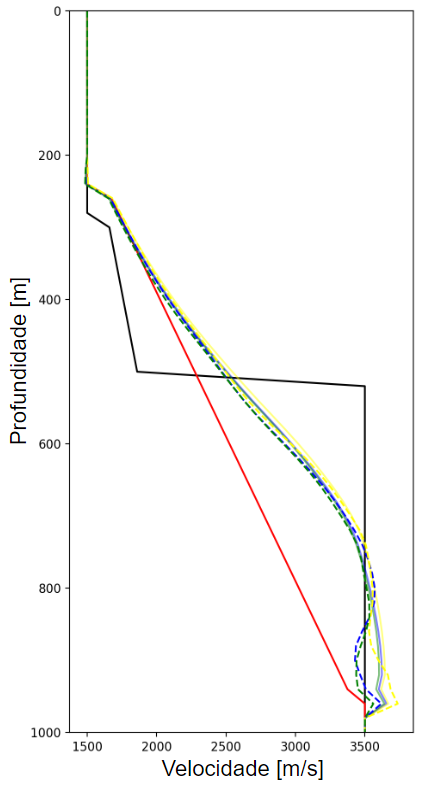
\includegraphics[width=3.2cm,height=6.5cm]{Imgs/Discussoes/upper_left_corner.png}}
	\subfloat[]{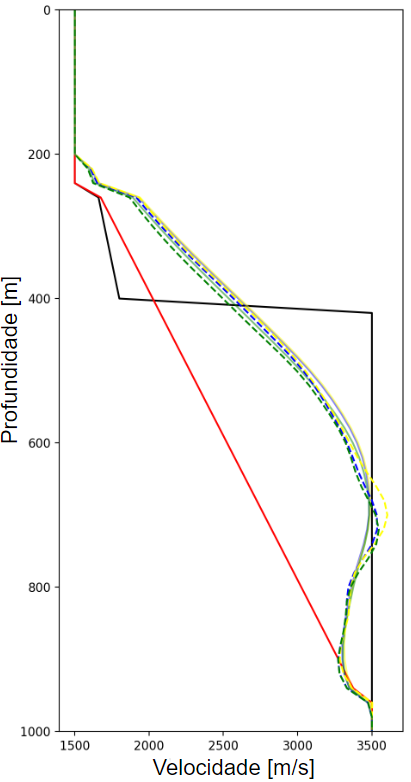
\includegraphics[width=3.2cm,height=6.5cm]{Imgs/Discussoes/lower_left_corner.png}}
	\subfloat[]{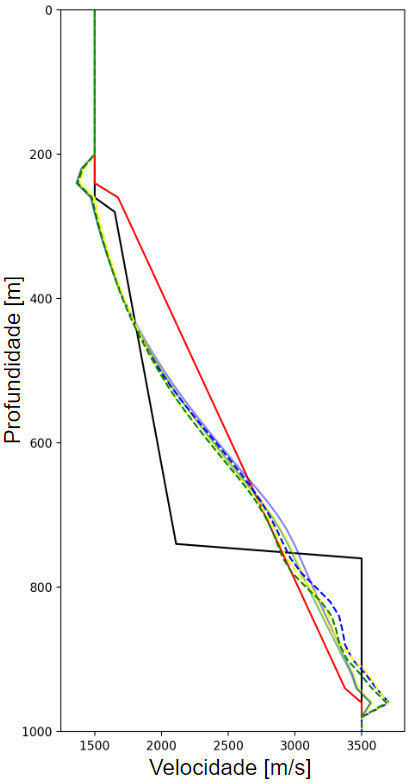
\includegraphics[width=3.2cm,height=6.5cm]{Imgs/Discussoes/center.png}}
	\subfloat[]{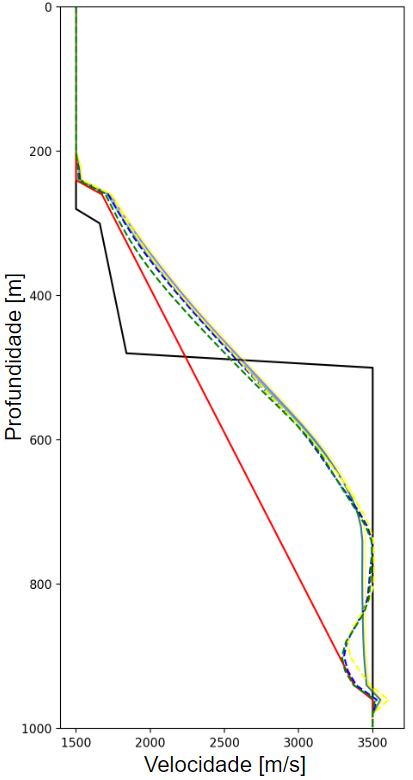
\includegraphics[width=3.2cm,height=6.5cm]{Imgs/Discussoes/upper_right_corner.png}}
	\subfloat[]{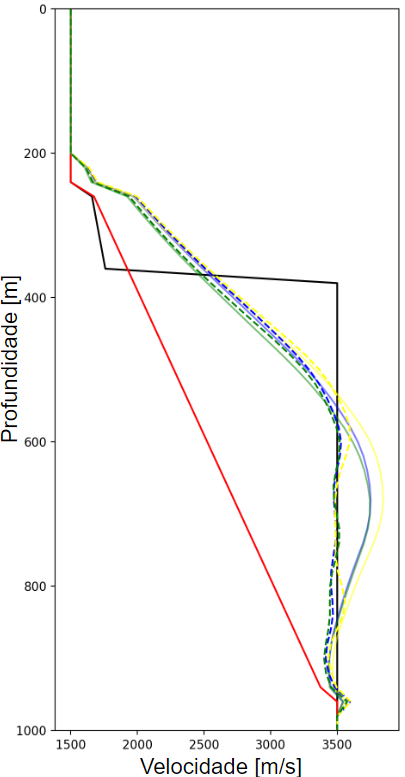
\includegraphics[width=3.2cm,height=6.5cm]{Imgs/Discussoes/lower_right_corner.png}}
	
	\caption{Modelos finais em forma de traço em cada posição central das gaussianas utilizadas. (a) Modelos projetados no ponto superior esquerdo. (b) Projeção no ponto inferior esquerdo. (c) Projeção central. (d) Projeção no ponto superior direito. (e) Projeção no ponto inferior direito. Em relação às cores, o modelo de referência se apresenta como o traço preto sólido e o modelo inicial como o traço vermelho sólido. Traços coloridos sólidos se referem aos modelos recuperados com malha esparsa e traços coloridos tracejados são modelos recuperados com malha refinada. A linha sólida preta é o modelo de referência e a vermelha é o modelo inicial. Os modelos recuperados a partir dos métodos estudados recebem as cores: azul para \citeonline{podvin1991finite}, amarela para \citeonline{jeong2008fast} e verde para \citeonline{jeong2008fast}. }
	\label{fig:model_profile}
\end{figure}

Os modelos apresentam boa correlação nas regiões fora da anomalia de alta velocidade, pois somente uma função de gradiente de velocidade foi corrigida onde variações pequenas, entre o modelo de referência e inicial, eram encontradas com relação à anomalia. Essas atualizações no modelo podem ser notadas nas Figuras \ref{fig:pod_refined}, \ref{fig:fim_refined} e \ref{fig:fsm_refined}, onde os modelos são ilustrados de forma regional. As correlações da velocidade próxima do horizonte do fundo marinho não foram satisfatórias, pois como o contraste regional é alto, os parâmetros de inversão empregados, como de regularização e discretização do modelo, privilegiaram as feições regionais deteriorando os detalhes do modelo recuperado. O ideal para corrigir os efeitos da topografia seria isolar o problema somente na parte do modelo onde existe o horizonte do fundo marinho e ajustar a sensibilidade dos parâmetros em relação à variação de velocidade no entorno da região alvo.  

Apesar dos modelos não apresentarem grandes diferenças em relação às velocidades recuperadas, a inversão utilizando modelagem da onda refratada com a formulação de \citeonline{jeong2008fast} mostra uma variação positiva de velocidade. Esse efeito pode ser explicado pelo atraso intrínseco nos tempos de trânsito da metodologia de modelagem, onde o modelo de velocidade se apresenta mais lento do que parece ser pelos altos tempos de trânsito calculados. Assim, por esse efeito, o esquema de inversão considera uma atualização mais rigorosamente alta na velocidade quando se utiliza a formulação de \citeonline{jeong2008fast}.    

